\documentclass[12pt,twoside]{article}   
\usepackage{light}
\usepackage{mathtools}
\newcommand{\defeq}{\vcentcolon=}
\newcommand{\eqdef}{=\vcentcolon}


\hidesolutions
\showsolutions
\newcommand{\proofrubric}[3][Any correct proof.]
  {
  	\begin{center}
	\fbox{\begin{minipage}{35em}
	\textbf{Rubric}
	\par
	[#3pts] #1
		\begin{center}
		\textbf{or}
		\end{center}
	#2
	\end{minipage}}
	\end{center}
  }
  
  \newcommand{\rubric}[1]
  {
  	\begin{center}
	\fbox{\begin{minipage}{35em}
	\textbf{Rubric}
	\par
	#1
	\end{minipage}}
	\end{center}
  }

\newcommand{\hint}[1]{({\it Hint: #1})}
\newcommand{\card}[1]{\left|#1\right|}

\begin{document}
\problemset{6}{October 13, 2016}{Thursday, October 20}
\noindent \textbf{Reading Assignment:}   Sections 5.4.3, 6.1, 6.2, 7.1-7.9
\\

%%%%%%%%%%%%%%%%%%%%%%%%%%%%%%%%%%%%%%%%%%%%%%%%%%%%%%%%%%%%%%%%%%%%%%%%%%%%%%%

% P3
\begin{problem}{20}

	This problem involves trees, which are a special class of graphs.  Suppose we consider a simple connected graph $G$ on $n$ nodes.  Then, $G$ is a tree if and only if $G$ is minimally connected (that is removing an edge disconnects $G$).

    \bparts
    
    \ppart{5} Show that our definition of a tree implies that a simple connected graph $G$ is a tree if and only if $G$ contains no cycles.
    \proofrubric{
    [2.5pts] Show that if $G$ contains a cycle, it is not minimally connected.\par
    [2.5pts] Contrapositive -- show that if $G$ is not minimally connected, then it contains a cycle.
    }{5}
    
    \solution{
    	Suppose that a simple connected graph $G$ is a tree, then we know by definition that it is minimally connected.  For the sake of contradiction, suppose that $G$ has a cycle and remove an edge $(u, v)$ in the cycle.  Now, we claim any two vertices $x, y$ in $G$ are still connected.  If $x, y$ were connected in $G$ by some path $p$ that did not use edge $(u, v)$, then they are still connected after removing edge $(u, v)$.  Now if path $p$ did contain edge $(u, v)$, then we replace the edge $(u, v)$ by the other longer path from $u$ to $v$ given by the cycle.  We now have a walk from $x$ to $y$, but now if there is a walk from $x$ to $y$, there must be a path and the graph is still connected after removing edge $(u, v)$, which is a contradiction.
    	
    	Now we show the other direction by proving the contrapositive.  That is, we want to show that if $G$ is not minimally connected, then it contains a cycle.  As $G$ is not minimally connected, there is some edge $e = (u, v)$ such that removing $e$ still leaves our graph connected.  Hence, there must be a path $p$ from $u$ to $v$ after removing edge $e$.  However, this means that the path $p$ along with edge $e$ forms a cycle, and so $G$ will contain a cycle. 
    }

    \ppart{5} Prove that a simple connected graph with $n$ nodes and $n-1$ edges is a tree.
\proofrubric{
[2pts] Proof by contradiction. Assume $G$ has a cycle. \par
[1pt] State that we want to show it is acyclic. \par
[2pts] Attempt to remove an edge and show it is not connected. \par
}{5}
    \solution{
        To show that a connected graph $G$ with $n$ nodes and $n-1$ edges is a tree, it is sufficient to show that it is acyclic. Assume to the contrary that there is a cycle in $G$; then we can remove an edge from this cycle while preserving connectivity. Then we have produced a connected subgraph $G'$ with $n$ vertices but only $n-2$ edges; this contradicts connectivity, and we conclude that the original graph must have been a tree.
    }
    
    \ppart{10} Prove that in any tree, any two longest paths cross each other (that is any two longest paths share a vertex).  
\proofrubric{
[2pts] Proof by contradiction. \par
[2pts] Assume two longest paths do not cross each other. \par
[2pts] Since trees are connected, there is some path between the two longest path. \par
[3pts] Show that the new longest path would be a combination of the two plus the path between the two.
}{10}
\solution{

	We prove this by contradiction.  Suppose that there are two longest paths in our tree that do not cross each other.  Let one path be from vertex $u$ to vertex $v$ and the other be from vertex $x$ to vertex $y$.  Then, as trees are connected, we must have that there is some vertex $a$ along the path from $u$ to $v$ that is connected to some vertex $b$ along the path from $x$ to $y$ by a path $p$ from $a$ to $b$ of length at least $1$.  Now, let $p_1$ be the longer of the paths from $u$ to $a$ and from $a$ to $v$.  Similarly, let $p_2$ be the longer of the paths from $x$ to $b$ and from $b$ to $y$.  Then each of the lengths of $p_1$, $p_2$ is at least half the length of the longest path.  Now consider the path $p_1 \cup p \cup p_2$.  As the length of $p$ is at least $1$, we have that the length of $p_1 \cup p \cup p_2$ is at least the length of the longest path plus $1$, which is a contradiction as this is now the longest path in the tree.

}

\eparts
\end{problem}


\begin{problem}{10}
    The adjacency matrix $A$ of a graph $G$ with $n$ vertices as defined in lecture is an $n \times n$
    matrix in which $A_{i,j}$ is 1 if there is an edge from $i$ to $j$ and 0 if there is not.
    In lecture we saw how 
    the smallest $k$ where $A^k_{i,j} \neq 0$ describes the length
    of the shortest path from $i$ to $j$. Give a combinatorial interpretation of the following statements about the adjacency matrix in terms of connectivity properties of $G$. For example, the smallest $k$ such that $A^k_{i,j}$ is non-zero means that the distance from $i$ to $j$ is at most $k$. 
\rubric{
For each: \par
    [3pts] Correct solution (all-or-nothing).
}
\bparts
\ppart{3}
    The trace of $A^{k}$ (the trace of a matrix is the sum of its diagonal entries).
    \solution{
	This is the number of closed walks of length $k$ in the graph $G$.  
    }

\ppart{2}
    $\forall k. A^{k}_{i,j} = 0$
    \solution{
        There is no path in $G$ from $i$ to $j$.
    }

\ppart{2}
    $\forall i \forall k. A^{k}_{i,i} = 0$
    \solution{
        The graph is acyclic. 
    }

\ppart{3}
$\forall k$, we can write $A^k$ as $\left[ \begin{array}{cc}
                                            X & 0 \\
                                            0 & Y 
                                    \end{array} \right]$
    \solution{
    There is no path from $X$ to $Y$ and so there are at least two connected components.
    }

\eparts
\end{problem}


\begin{problem}{15}
A set of PageRank values is stationary if the amount of PageRank going into each vertex is the same
as the amount leaving the vertex on every update.
In this problem we will prove that a strongly connected graph has at most one set of PageRank values that are stationary. There always is a set of PageRank values that are stationary, but
we are not asking you prove this.

\bparts

\ppart{7}
  For two sets of values of PageRank, $d_1$ and $d_2$, let $\gamma$ be defined as 
  $\gamma \vcentcolon \max_{x \in V} \frac{d_1(x)}{d_2(x)}$, the maximum ratio
  of a value in $d_1$ over the corresponding value in $d_2$.
  Show that there exists a directed edge from $y$ to $z$ such that
  $d_1(y)/d_2(y) < \gamma$ and $d_1(z)/d_2(z) = \gamma$.
\rubric{
[3pts] Argue that ration of < $\gamma$ has to exist otherwise values would be the same.\par
[4pts] Show why being strongly connected is necessary. Give 2 or 3 points if they mention something about vertices being connected.
}
\solution{
  $\gamma$ must be attained at some vertex and not all vertices have 
  a ratio of $\gamma$ because if they did then the
values would be the same.
  Because the graph is strongly connected, we can follow edges backwards until we 
  arrive at any other vertex and there must be some
  vertex along the way that does not attain $\gamma$.
  So such an edge must exist.
}

\ppart{8}
  Prove that a strongly connected graph has at most one set of PageRank
values that are stationary by deriving a contradiction using the edge
  found in part a.

\proofrubric{
[2pts] $d_1$ and $d_2$ are stationary at $z$\par
[3pts] Apply a step of page rank\par
[3pts] Correct math for deriving a contradiction. \par
[-1pt] Math errors.
}{8}

\solution{
  Assume for the sake of contradiction that there are two stationary
values $d_1$ and $d_2$.  Let $\gamma$ be defined as 
  $\gamma \eqdef \max_{x \in V} \frac{d_1(x)}{d_2(x)}$, the maximum ratio
  of a value in $d_1$ over the corresponding value in $d_2$.

  Pick an edge from $y$ to $z$ such that
  $d_1(y)/d_2(y) < \gamma$ and $d_1(z)/d_2(z) = \gamma$.
  $\gamma$ must be attained at some vertex and not all vertices have 
  a ratio of $\gamma$ because if they did then the
values would be the same.
  Because the graph is strongly connected, we can follow edges until we 
  arrive at any other vertex and there must be some
  vertex along the way that does not attain $\gamma$.
  So such an edge must exist.

  Define $p(x,z)$ to be $\frac{\text{Number of edges from x to z}}{\text{Number of edges out of x}}$
  We apply one step of PageRank to $d_1$ and $d_2$ which are stationary values $\widehat{d_1}$ and $\widehat{d_2}$.
  \begin{equation}\label{d1}
    d_1(z) = \widehat{d_1}(z) = \sum_{x: x\rightarrow z} d_1(x) p(x,z),
  \end{equation}
  and
  \begin{equation}\label{d2}
    d_2(z) = \widehat{d_2}(z) = \sum_{x: x\rightarrow z} d_2(x) p(x,z).
  \end{equation}

  Substituting $d_1(z) = \gamma d_2(z)$ into \eqref{d1}, and recalling
  that $d_1(x) \leq \gamma d_2(x)$ for all $x$, we have
  \begin{align*}
    \gamma d_2(z)
        &= \sum_{x: x\rightarrow z} d_1(x) p(x,z) \\
        &= \paren{\sum_{x \neq y: x\rightarrow z}
          d_1(x)p(x,z)} + d_1(y) p(y,z) \\
        &\leq \paren{\sum_{x \neq y: x\rightarrow z} \gamma d_2(x)
          p(x,z)} + d_1(y) p(y,z) \\
        &\leq \paren{\paren{\gamma \sum_{x: x\rightarrow z} d_2(x)
          p(x,z)} - \gamma d_2(y)p(y,z)} + d_1(y) p(y,z) \\
        &\leq \gamma d_2(z) - \gamma d_2(y)p(y,z) + d_1(y) p(y,z)\\
        &< \gamma d_2(z) - \gamma d_2(y)p(y,z) + \gamma d_2(y) p(y,z)\\
        &< \gamma d_2(z).
  \end{align*}
  The strict inequality at the next to last step of the derivation
  follows from the assumption that $d_1(y) < \gamma d_2(y)$, and
  $p(y,z) > 0$.  Thus, we have shown $d_2(z) < d_2(z)$, which is a
  contradiction.
}

\eparts

\end{problem}


%%%%%%%%%%%%%%%%%%%%%%%%%%%%%%%%%%%%%%%%%%%%%%%%%%%%%%%%%%%%5555


\begin{problem}{15} 

\bparts

\ppart{5}
    For the graph in Figure~\ref{scc-graph}, compute the first two iterations
    of PageRank, starting from uniform PageRank values across all vertices.

    \begin{figure}[h!]
    \begin{center}
        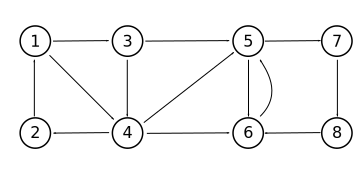
\includegraphics{ps6-scc-graph.pdf}
        \caption{A graph of web pages and links.}
        \label{scc-graph}
    \end{center}
    \end{figure}

\rubric{
[-0.5pts] Each incorrect vertex in iter 2. \par
[-5pts] Obviously incorrect methodology.
}
    \solution{
        In the table below, we write the PageRank value of each vertex at
        iterations $0$, $1$, and $2$. We also include, for each vertex, the
        individual contributions made to that vertex in computing the next
        stage, which are summed in computing the following PageRank value.

        \begin{center}
        \begin{tabular}{r|cccccccc}
            & 1 & 2 & 3 & 4 & 5 & 6 & 7 & 8 \\
            \hline \\[-0.5em]
            iter 0  & $\frac18$ & $\frac18$ & $\frac18$ & $\frac18$ & $\frac18$ & $\frac18$ & $\frac18$ & $\frac18$ \\[1em]
            contrib & $\frac18$ & $\frac1{24}$ & $\frac1{16}$ & $\frac1{16}, \frac18$ & $\frac18, \frac1{16}, \frac1{24}$ & $\frac18, \frac1{16}, \frac1{24}$ & $\frac1{16}$ & $\frac18$ \\[1em]
            iter 1  & $\frac18$ & $\frac1{24}$ & $\frac1{16}$ & $\frac18$ & $\frac{11}{48}$ & $\frac{11}{48}$ & $\frac1{16}$ & $\frac18$ \\[1em]
            contrib & $\frac1{24}$ & $\frac1{24}$ & $\frac1{16}$ & $\frac1{16}, \frac1{32}$ & $\frac1{24}, \frac1{32}, \frac{11}{48}$ & $\frac18, \frac1{24}, \frac{11}{96}$ & $\frac{11}{96}$ & $\frac1{16}$ \\[1em]
            iter 2  & $\frac1{24}$ & $\frac1{24}$ & $\frac1{16}$ & $\frac3{32}$ & $\frac{29}{96}$ & $\frac{9}{32}$ & $\frac{11}{96}$ & $\frac1{16}$ 
        \end{tabular}
        \end{center}
    }

\ppart{10}
    A strongly connected component of a directed graph is a subgraph which
    has the property that for every pair of vertices 
    $u$ and $v$, there exists a path from
    $u$ to $v$ and one from $v$ to $u$. Also, every vertex which can be
    reached by a path starting in the strongly connected component is also
    in the strongly connected component.
    Suppose that a graph $G$ consists of exactly two strongly connected
    components $C_1$ and $C_2$, and that there exist edges from $C_1$ to
    $C_2$ (but not from $C_2$ to $C_1$). There is always a stationary set of
    values which is non-negative. Prove that the stationary PageRank 
    values of this graph are entirely concentrated in $C_2$, i.e.\ that the
    PageRank values are all zero on $C_1$.
\proofrubric{
[2pts] Proof by contradiction. \par
[2pts] Contradiction is in whether PageRank values are stationary. \par
[2pts] Use a vertex in $C_1$ that has an edge to $C_2$. \par
[2pts] Show vertex has contributions to it. \par
[2pts] No contributions from $C_2$ to $C_1$ so not stationary.
}{10}
    \solution{
        For any vertex $v$, let $p(v)$ denote the stationary PageRank value
        at $v$, so that if we apply another step of the PageRank update rule
        to these values, they remain unchanged.  Suppose for a contradiction
        that for some vertex $v \in C_1$, $p(v) \neq 0$.

        Let $w$ be any other vertex of $C_1$; we first claim that the PageRank
        value at $w$ is positive. From the hypothesis that $C_1$ is strongly
        connected, there exists a path from $v$ to $w$, of some length $k$. If
        we were to apply $k$ steps of the PageRank algorithm, then
        the non-zero PageRank value $p(v)$ would yield some positive
        contribution to the resulting value at $w$, via the path mentioned
        above. The resulting PageRank value at $w$ after $k$ steps would then
        be positive. As the PageRank values were already stationary we
        can conclude that $p(w) > 0$.

        Now, we know that some vertex $w \in C_1$ has an edge leading into
        $C_2$. As the PageRank value $p(w)$ is positive, then if we were to
        apply another step of the PageRank update rule, vertex $w$ would make
        a contribution of at least $\frac{p(w)}{\mathrm{outdeg}(w)}$ to the
        total PageRank of component $C_2$. There are however no edges from
        $C_2$ to $C_1$. As the total PageRank in a graph always sums to $1$,
        we must conclude that the total PageRank in component $C_1$ decreases
        by at least $\frac{p(w)}{\mathrm{outdeg}(w)} > 0$ by applying the
        update rule.

        But these PageRank values were assumed to be stationary, and we
        have argued above that they must change when we apply the update step.
        This is a contradiction, and so the stationary PageRank values must
        be zero throughout component $C_1$, as desired.
    }

\eparts

\end{problem}



%-----------------------------------------------------------------%
% source: Velleman 4.6, Exercise 3.
% topic: equivalence relations
% last used Fall00 Problem Set 3 (in ProblemRepository)

% In 2010 and 2012

\begin{problem}{10}
For each of the following, either prove that it is an equivalence relation and state its equivalence classes, or give an example of why it is not an equivalence relation. 
\rubric{
For each: \par
[1pt] Correct true/false for equivalence relation. \par
[1pt] Correct counterexample or proof. \par
}
\bparts
\ppart{2}
$R_n := \{(x, y) \in \mathbb Z \times \mathbb Z \textrm{ s.t. } x \equiv y \pmod n \}$
\solution{
	It is an equivalence relation.  To prove this, we will show that $R_n$ is symmetric, transitive, and reflexive.
	\begin{itemize}
		\item
			\textbf{Reflexive}: $x \equiv x \pmod n$.  This is because $x = x + 0 \cdot n$.  
		\item 
			\textbf{Symmetric}: We want to show that $R_n(x, y) \Rightarrow R_n(y, x)$.  If $R_n(x, y)$, then there is some $c \in \mathbb Z$ such that $x = y + c \cdot n$.  But then,
				subtracting $c \cdot n$ from both sides, we have that $y = x + (-c) \cdot n$, so $y \equiv x \pmod n$.  So $R_n(y, x)$, and the symmetric property holds.
		
		\item
			\textbf{Transitivity}.  Suppose $R_n(x, y)$ and $R_n(y, z)$.  From the first statement, we know that there is some $c \in \mathbb Z$ such that $x = y + c\cdot n$.  From the second,
			we know that there is some $d \in \mathbb Z$ such that $y = z + d \cdot n$.  Substituting in this value of y, we see that $x = (z + d \cdot n) + c \cdot n = z + (d + c) \cdot n$.  The
			sum $c + d$ is an integer, so $R_n(x, z)$ holds.  
	\end{itemize}
	The equivalence classes are then the sets of numbers congruent to the numbers $\{0, 1, \ldots, n-1 \}$ modulo n.
}

\ppart{2}
$R := \{ (x, y) \in P \times P \textrm{ s.t. } x \textrm{ is taller than } y \}$
where $P$ is the set of all people in the world today.
\solution{
	This is not an equivalence relation, because the concept of symmetry is broken.  If $y$ is taller than $x$, then $x$ is not taller than $y$.
}

\ppart{3} 
$R := \{ (x, y) \in \mathbb Z \times \mathbb Z \textrm{ s.t. } gcd(x,y)=1 \}$
\solution{
	This is not an equivalence relation, because transitivity is broken.  Consider the case when $x = 3$, $y = 7$, and $z = 15$.  Then, $gcd(x,y)=1$ and $gcd(y,z)=1$, but $gcd(x,z)=3\neq 1$.
}

\ppart{3}
$R_G := $ the set of $(x, y) \in V \times V$ such that $V$ is the set of vertices of a graph $G$, and there is a path $x, v_1, \ldots, v_k, y$ from $x$ to $y$ along the edges of $G$.

\solution{
	This is an equivalence relation.  We will show this by proving that it obeys reflexivity, symmetry, and transitivity.
	\begin{itemize}
	\item
		\textbf{Reflexivity}: Any vertex is connected to itself.  
	\item
		\textbf{Symmetry}: If $R_G(x, y)$, then there is a path $x, v_1, \ldots, v_k, y$ from $x$ to $y$.  The reverse of this path is $y, v_k, \ldots, v_1, x$, and is a path from
		$y$ to $x$.  So $R_G(y, x)$.
	\item
		\textbf{Transitivity}:  Suppose $R_G(x, y)$ and $R_G(y, z)$.  Then, there is a path from $x$ to $y$: $x, v_1, \ldots, v_k, y$.  Furthermore, there is a path from $y$ to $z$: 
		$y, w_1, \ldots, w_l, z$.  But then, the concatenation of those two is a path $x, v_1, \ldots, v_k, y, w_1, \ldots, w_l, z$ from $x$ to $z$.  So $R_G(x, z)$.
	\end{itemize}
	
	Thus we have shown that $R_G$ is an equivalence relation on a graph $G$, and the equivalence classes are the connected components of $G$.
}

\eparts
\end{problem}


%%%%%%%%%%%%%%%%%%%%%%%%%%%%%%%%%%%%%%%%%%%%%%%%%%%%%%%%%%%%%%%%%%%%%%%%%%%%%%


\begin{problem}{10}
Let $R_1$ and $R_2$ be two equivalence relations on a set, $A$.  Prove
or give a counterexample to the claims that the following are also
equivalence relations:

\bparts

\ppart{5} 
$R_1 \cap R_2$.
\rubric{
[1pt] Is an equivalence relation. \par
[4pts] Correct proof. \par
}
\solution{
Let $R \eqdef R_1 \cap R_2$.  We give two proofs that $R$ is an
equivalence relation using different characterizations of equivalence
relations.

\begin{proof}
We first prove that $R$ is an equivalence relations by showing that $R$ is
reflexive, symmetric, and transitive.

\emph{Reflexive:} $R_i$ is reflexive because it is an equivalence
relation, for $i=1,2$.  So $(a,a) \in R_i$ for $i=1,2$ and all $a \in A$.
So, $(a,a) \in (R_1 \cap R_2) = R$ for all $a \in A$, that is, $R$
is reflexive.

\emph{Transitive:} Suppose $(a,b), (b,c) \in R$.  Since $R = R_1
\cap R_2$, we have $(a,b), (b,c) \in R_i$ for $i=1,2$.  But $R_i$ is
an equivalence relation, and so is transitive.  Therefore, $(a,c) \in
R_i$, and so $(a,c) \in R_1\cap R_2 = R$.  This shows that $R$ is
transitive.

\emph{Symmetric:} The proof that $R$ is symmetric follows the same format.

\end{proof}

\begin{proof}
Since $R_i$ is an equivalence relation for $i=1,2$, there is by
definition a total function, $f_i$, with domain, $A$, such that
\[
aR_i b \quad\text{ iff }\quad f_i(a) = f_i(b).
\]
Define the function, $f$, with domain, $A$, by
\[
f(a) \eqdef (f_1(a),f_2(a)).
\]
Clearly $f$ is total, since $f_i$ is total for $i=1,2$.  Now we have,
\begin{align*}
aRb \quad &  \text{ iff }\quad a(R_1 \cap R_2)b & \text{def.\ of $R$}\\
    &  \text{ iff }\quad aR_ib\text{ for }i=1,2 & \text{def.\ of $\cap$}\\
    &  \text{ iff }\quad f_i(a)=f_i(b) \text{ for }i=1,2 & \text{def.\ of $f_i$}\\
    &  \text{ iff }\quad (f_1(a),f_2(a)) = (f_1(b),f_2(b)) & \text{def.\ of $=$ pairs}\\
    &  \text{ iff }\quad f(a) = f(b) & \text{def.\ of $f$}.
\end{align*}
That is
\[
aRb \quad \text{ iff }\quad f(a) = f(b),
\]
which proves that $R$ is the equivalence relation $\equiv_f$.
\end{proof}
}


\ppart{5}
$R_1 \cup R_2$.
\rubric{
[1pt] Is not an equivalence relation. \par
[4pts] Correct counterexample. \par
}
\solution{
We give a counterexample showing that $R_1 \cup R_2$ may not be
an equivalence relation.  Let $R_1$ and $R_2$ be the relations on
$\set{1, 2, 3}$ where
\begin{align*}
R_1 \eqdef & \set{(1,1) (2,2) (3,3) (1,2) (2,1)},\\
R_2 \eqdef & \set{(1,1) (2,2) (3,3) (2,3) (3,2)}.
\end{align*}
It's easy to check that $R_1$ and $R_2$ are both equivalence relations.
But $R_1\cup R_2$ is not transitive, because $(1,2),(2,3) \in R_1\cup R_2$
and $(1,3) \notin R_1\cup R_2$.  Therefore $R_1\cup R_2$ is not an
equivalence relation.
}

\eparts

\end{problem}


%%%%%%%%%%%%%%%%%%%%%%%%%%%%%%%%%%%%%%%%%%%%%%%%%%%%%%%%%%%%%%%%%%%%%%%%5


\begin{problem}{20}
In this problem we study partial orders (posets). Recall that a weak partial order $\preceq$ on a set $X$ is reflexive $(x \preceq x)$, anti-symmetric ($x \preceq y \wedge y \preceq x \rightarrow x = y$), and transitive ($x \preceq y \wedge y \preceq z \rightarrow x \preceq z$). Note that it may be the case that neither $x \preceq y$ nor $y \preceq x$. A chain is a list of {\it distinct} elements $x_1, \ldots, x_i$ in $X$ for which $x_1 \preceq x_2 \preceq \cdots \preceq x_i$. An antichain is a subset $S$ of $X$ such that for all distinct $x, y \in S$, neither $x \preceq y$ nor $y \preceq x$. 

\bparts

\ppart{10}  A chain in a poset is called maximal if it cannot be extended (that is no other element of the poset can be added to it).  Let $B_4$ (the Boolean algebra) be the set of subsets of $\{ 1, 2, 3, 4 \} $ where the partial order is defined by the contains operation (the number of elements in $B_4$ is $2^4$ and for subsets $S_1, S_2$, $S_1 < S_2$ if $S_1 \subset S_2$).  How many maximal chains does $B_4$ have?
\proofrubric[24 or 4!]{
[-1pt] Math errors. \par
[5pts] Use definition of maximal by extending a chain.\par
[5pts] Permutation on the elements that can be added to the chain. \par
}{10}
\solution{

$B_4$ should have $4! = 24$ maximal chains.  Let us consider the general case of $B_n$ and show that $B_n$ has $n!$ maximal chains.  Note that if we have some non-maximal chain, we can always extend it by adding a new element to the largest subset in the chain if the largest element is not $\{1, 2, \ldots n\}$ or by removing an element from the smallest subset in the chain if the smallest element is not $\emptyset$.  Hence,  to find all maximal chains, let us being with $\emptyset$ and add elements to our chain until we reach $\{1, 2, \ldots n\}$.  We have $n$ choices for our first extension to our chain, $n-1$ choices for the second extension and so on until we are left with exactly $1$ choice to extend our chain to $\{1, 2, \ldots n\}$.  Hence there are $n!$ maximal chains, and so for $B_4$ there are 24.

}

\ppart{10} Let $\pi$ be a permutation, and let $d$ be the smallest integer so that $\pi$ can be written as a union of $d$ increasing sequences.  Prove that the longest decreasing subsequence of $\pi$ consists of $d$ elements.  (Hint: use Dilworth's theorem) 
\proofrubric{
[3pts] Define a partial order for the poset. \par
[3pts] Chains in poset are increasing subsequences. \par
[3pts] Antichains correspond to decreasing subsequences. \par
[1pt] Dilworth's theorem.
}{10}
\solution{

This is actually a special case of Dilworth's theorem.  We just need to define the appropriate partial order $<_P$ for our poset $P$.  Let $\pi = \pi_1 \pi_2 \ldots \pi_n$.  Then we say that $\pi_i <_P \pi_j$ if $\pi_i < \pi_j$ and $i < j$.  Then the chains of our poset $P$ are the increasing subsequences in $\pi$ and so antichains of $P$ correspond to decreasing subsequences in $\pi$.  The proof then follows by Dilworth's theorem.  
}

\eparts

\end{problem}



%%%%%%%%%%%%%%%%%%%%%%%%%%%%%%%%%%%%%%%%%%%%%%%%%%%%%%%%%%%%%%%%%%
\end{document}
